%\chapter{Rayonnement électromagnétique}
%\section{Introduction historique}
%Un peu plus de 10 ans après la publication des lois de Maxwell, Hertz réalise une expérience qui a permis de mettre en évidence l'existence de ce que ce-premier avait prévu mathématiquement, les ondes électromagnétiques que nous désignerons par ondes E.M. L'expérience de Hertz invoquait un "\textit{oscillateur}" LC produisant des arcs électriques à un intestice appelé éclateur. \footnote{Il utilisait pour cela une bobine de Ruhmkorff munie d'un condensateur. Celle-ci se base sur le même principe que les transformateurs actuels à ceci près qu'à son entrée, seule une alimentation continue était requise : \url{https://en.wikipedia.org/wiki/Induction_coil}.} ainsi qu'un récepteur que nous pourrions appeler un "\textit{résonateur}" de Hertz. Ce dernier était une boucle conductrice formant un inducteur mais gardant un interstice d'éclatement et une capacité réglable : un sorte de second "\textit{oscillateur}". \\Lorsque le premier "\textit{oscillateur}" était en fonctionnement, Hertz s'est aperçu que lorsqu'il plaçait la boucle du "\textit{résonateur}" selon une certaine configuration par rapport à l'éclateur, sans la moindre connection électrique, d'autres arcs électriques apparaissaient aux bornes de l'éclateur du "\textit{résonateur}" (voir \ref{fig:expHertz}). Il mit également en évidence le concept de polarisation des ondes E.M. en inclinant autrement son "\textit{résonateur}" par rapport à l'éclateur primaire, les arcs électriques pouvaient disparaître (sur le schéma, il s'agirait du cas où le champ $\vec{\mathcal{H}}$ et ses variations ne sont plus interceptées par la spire du "\textit{résonateur}"). \\
%Le système de condensateur à base de sphères chargées utilisé par Hertz seront traités dans le cadre du cours de Physique 3 comme des charges ponctuelles qui se déplacent de haut en bas et et bas en haut. L'ensemble forme donc un dipôle oscillant.
%\begin{figure}[h]
%\begin{minipage}[l]{.5\linewidth}\centering
%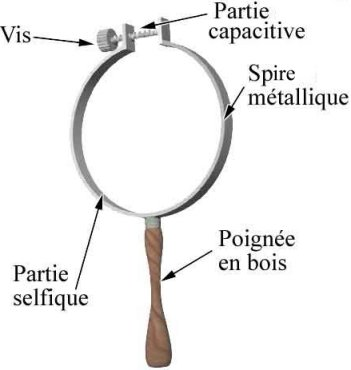
\includegraphics[height=5cm]{hertz1}
%\caption{Récepteur de Hertz}
%\end{minipage}
%\begin{minipage}[]{.5\linewidth}\centering
%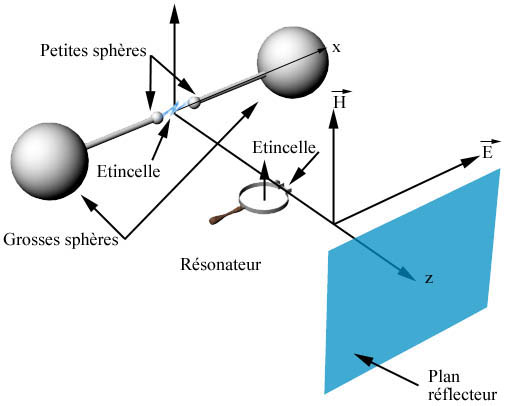
\includegraphics[height=5cm]{hertz2}
%\label{fig:expHertz}
%\caption{Expérience de Hertz} 
%\end{minipage}
%\end{figure}
%
%\subsection{Physique du rayonnement}
%Ce paragraphe introductif est hors-matière mais traite de l'intuition qui se cache derrière les champs rayonnés : il se réfère aux lectures supplémentaires disponibles sur le site du cours. \\ \\
%A l'instar du concept de particule chargée au repos dans un référentiel galiléen classique créant un champ électrique statique et à l'instar du même genre de particule mais cette fois-ci en mouvement à vitesse constante uniforme générant un champ magnétique, lorsque la particule est accélérée il se développe alors ce que nous appelons un champ rayonné : une onde électromagnétique. Ce champ rayonné intégrera donc bien un couplage entre champ magnétique et champ électrique. \\ \\
%Nous nous proposons ici d'expliquer brièvement en quoi, lorsqu'une charge est accélérée, un phénomène de radiation apparaît. L'idée est la suivante. Il est tout d'abord nécessaire de s'imaginer un champ électrique statique associé à une charge au repos. Admettons que pour une certaine raison, elle soit accélérée uniformément selon la direction $\hat{x}$ du référentiel considéré avec une intensité $a$ pendant un temps $\tau$ à partir de $t = 0$. Après, pour $t>\tau$, l'accélération cesse et la particule continue son bonhomme de chemin à une allure constante $v = a\,\tau$ selon $\hat{x}$. A vitesse constante, la particule développe non seulement un champ magnétique mais également un champ électrique non-plus statique mais en mouvement ; en vulgarisant quelque peu, "\textit{centré et attaché}" à la particule. En considérant les temps $t = 0$ et $t = \tau$, nous observons aisément que le champ électrique associé à la particule chargée n'est pas centré au même endroit : il a non seulement été projeté en avant suite au mouvement de la particule mais ce de manière plus rapide que la vitesse initiale constante de déplacement du champ électrique jusque là (accélération). Le développement suivi ici est donc valable pour toute accélération de la particule chargée : qu'importe sa vitesse initiale. Cependant, et c'est là où réside toute l'essence même du rayonnement, ce changement de \textit{centrage} ne s'opère pas de manière instantanée! La figure \ref{fig:yo} montre bien que "\textit{l'information physique}" se propage à vitesse finie ($c = \frac{1}{\sqrt{\epsilon\,\mu}} < \infty $) vers l'extérieur.
%\begin{figure}[h]
%\centering
%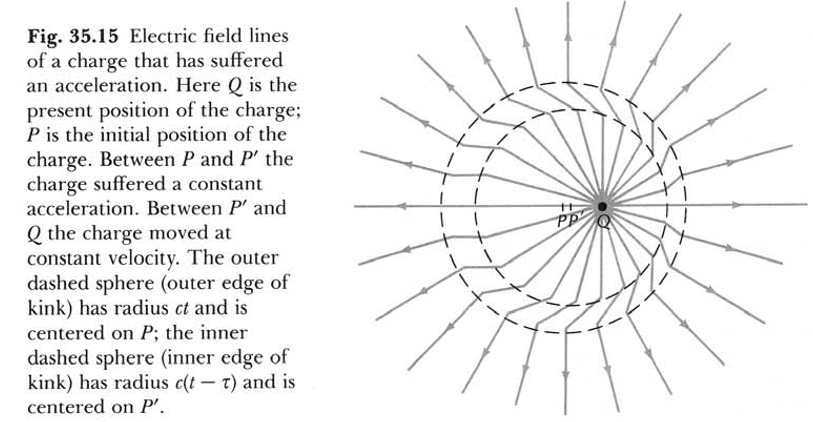
\includegraphics[height=5cm]{figure.PNG}
%\caption{Illustration du changement de \textit{centrage} et propagation du signal (tirée des lectures complémentaires)}
%\label{fig:yo}
%\end{figure}
%
%
%\newpage 
%
%En première approximation, nous pouvons tracer des traits entre les lignes du nouveau champ électrique s'établissant progressivement et un champ électrique issu de temps antérieurs. Nous pouvons nous figurer que lorsque l'accélération cesse, tous ces changements cessent également et aucune "\textit{information}" supplémentaire sur la nature  du champ ne se propage. Cette "\textit{information}" dont nous traitons depuis quelques lignes n'est rien d'autre qu'un champ électrique rayonné qui vient se superposer au champ électrique latent afin que le champ électrique total résultant tende à se calquer vers un champ électrique plus actuel (comprendre : associé à la particule chargée en un temps postérieur). \\ \\Sans rentrer dans les détails d'un développement mathématique fastidieux, forts de ce constat, nous pouvons avancer que l'évolution du champ rayonné en un point de l'espace $\vec{r}$ dépend non pas du temps actuel $t$ mais bien du temps $t' = t - \frac{|| \vec{r} - \vec{r}_{p} ||}{c}$ qu'il était lorsque l'accélération instantanée (menant à la propagation d'un front d'onde comme sur la figure \ref{fig:yo}) tint lieu. En effet, il faut tenir compte du déphasage temporel $\frac{||\vec{r} - \vec{r}_{p} ||}{c}$ lié au temps mis par le front d'onde pour arriver en $\vec{r}$ depuis $\vec{r}_{p}$ (position où l'accélération a été subie). \\ \\
%Aussi, intuitivement, nous accepterons pour la suite du document que l'amplitude du champ rayonné est directement proportionnelle à l'accélération subie. En effet, admettons que celle-ci soit minuscule : en repartant de notre scénario initial, la particule chargée avancera à peine et ce de manière très lente, le champ rayonné afin d'homogénéiser l'espace entier par rapport à un nouveau champ électrique issu de la particule s'étant déplacée sera de très faible amplitude car peu de choses auront réellement changé. De plus, si jamais nous avions considéré une accélération dans le sens opposé, il est clair que le schéma de la figure \ref{fig:yo} aurait simplement subi une symétrie axiale.\\ Désormais, il va nous falloir admettre un postulat ; confirmé par la figure \ref{fig:yo} si nous regardons dans la direction de l'accélération. Il s'agit d'observer que seule la composante orthogonale de l'accélération en $t'$ par rapport à la position $\vec{r}$ considérée entraîne un rayonnement. Cet effet est illustré à la figure \ref{fig:yo2} directement prélevée des slides du cours. A la figure \ref{fig:yo}, nous imaginons déjà qu'aucun champ rayonné n'apparaît dans la direction $\hat{x}$ puisqu'il n'y a pas de déformation de la ligne de champ dans cette même direction.  \\ \\
%Enfin, puisque la puissance du signal (champ électrique) se propageant doit être conservée et qu'il se propage dans toutes les directions \footnote{Nous verrons qu'il faut être prudent en disant cela : certaines directions se verront doter d'une propagation de champ rayonné d'amplitude nulle. Il est ici juste nécessaire de saisir les idées sous-jacentes.}, il faut savoir que l'intensité ([$W/m^{2}$]) du champ rayonné sera proportionnelle à $\frac{1}{|| \vec{r} - \vec{r}_{p} ||^{2} }$ puisque le front d'onde décrit successivement des boules centrées en $\vec{r}_{p}$ d'enveloppe de surface évoluant avec le carré du rayon. Attendu que, comme nous avons pu le découvrir, l'intensité est directement liée au carré de l'amplitude du champ électrique associé ; cette dernière sera proportionnelle à $\frac{1}{||\vec{r} - \vec{r}_{p}||}$ = $r'$ .
%\newpage
%\begin{figure}[h]
%\centering
%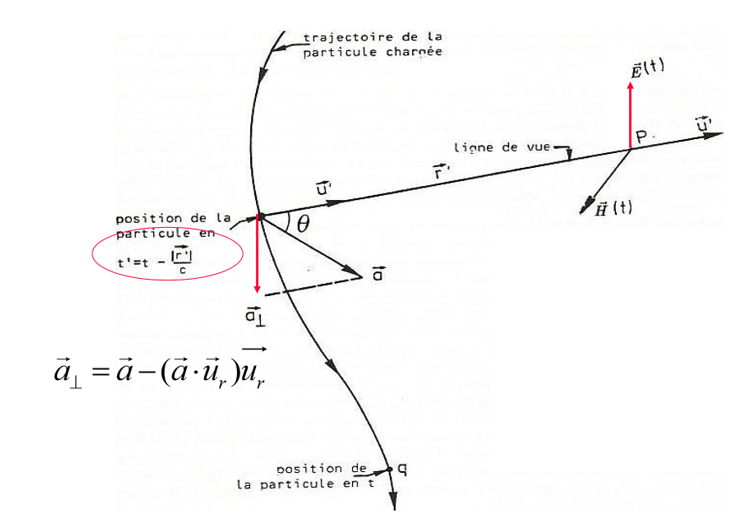
\includegraphics[height=8cm]{lol2.PNG}
%\caption{Illustration du postulat}
%\label{fig:yo2}
%\end{figure} 
%
%Au final, en combinant toutes les observations et les hypothèses émises, nous formulons que l'amplitude du champ électrique  rayonné\footnote{Lorsque ce champ électrique rayonné variera dans le temps, là apparaîtra ce fameux couplage à un champ magnétique formant, à deux, une onde E.M. Nous y reviendrons.} suit une relation de proportionnalité du type\footnote{Bien entendu, $\vec{E}_{r}$ est proportionnel à la charge électrique en mouvement.} : 
%\[ \vec{E}_{r}(\vec{r},t) \propto \frac{q}{r'}\,\vec{a}_{\perp}(t' = t - \frac{||\vec{r}-\vec{r}_{p}||}{c})\] 
%
%Dans la suite du document, plusieurs abus de notations / simplifications seront utilisés. \\ \\ Premièrement, nous parlerons souvent de champ électrique (sous-entendu : total) à la place de champ électrique rayonné. Cela vient du fait que selon la loi de Coulomb traditionnelle, l'amplitude des champs électriques statiques (ou se déplaçant à vitesse constante) sont, à tout instant, inversement proportionnels au carré de la distance qui sépare un point considéré de l'espace vis à vis du centre (la charge). Le champ rayonné quant à lui est "\textit{seulement}" inversement proportionnel à la distance tout court. Autrement dit, lorsque nous sommes relativement éloignés du "\textit{centre}", c'est à dire de la source ponctuelle de champ électrique (particule chargée), l'amplitude du champ électrique de base tend très rapidement vers des quantités tout à fait négligeables devant l'amplitude du champ rayonné ; voilà pourquoi, à distance convenable, nous marquerons souvent : \[\vec{E} \simeq \vec{E}_{r}\] 
%Secondement, parfois, certaines formules ne feront pas la distinction entre $t$ et $t'$. \\\\
%Enfin, attendu que nous considérerons toujours un dipôle oscillant comme la base de nos champs rayonnés et que les particules chargées dans ce cas là bougent le long d'un axe (antenne) sur de très courtes distances généralement, nous admettrons souvent que $\vec{r}_{p} \simeq \vec{0}$.\footnote{Une explication plus formelle est disponible dans les notes complémentaires du cours. A nouveau, ce n'est pas matière de l'examen. Il est néanmoins intéressant de les lire. Une animation est disponible sur ce site pour mieux visualiser le phénomène de rayonnement : \url{http://www.tapir.caltech.edu/~teviet/Waves/empulse.html}}
% 
% \newpage 
% 
\chapter{Rayonnement électromagnétique}
\section{Introduction historique}
Un peu plus de 10 ans après la publication des lois de Maxwell, Hertz réalise une expérience qui a permis de mettre en évidence l'existence de ce que ce-premier avait prévu mathématiquement, les ondes électromagnétiques que nous désignerons par ondes E.M. L'expérience de Hertz invoquait un "\textit{oscillateur}" LC produisant des arcs électriques à un interstice appelé éclateur. \footnote{Il utilisait pour cela une bobine de Ruhmkorff munie d'un condensateur. Celle-ci se base sur le même principe que les transformateurs actuels à ceci près qu'à son entrée, seule une alimentation continue était requise : \url{https://en.wikipedia.org/wiki/Induction_coil}.} ainsi qu'un récepteur que nous pourrions appeler un \textit{résonateur}" de Hertz. Ce dernier était une boucle conductrice formant un inducteur mais gardant un interstice d'éclatement et une capacité réglable : une sorte de second "\textit{oscillateur}". \\Lorsque le premier "\textit{oscillateur}" était en fonctionnement, Hertz s'est aperçu que lorsqu'il plaçait la boucle du "\textit{résonateur}" selon une certaine configuration par rapport à l'éclateur, sans la moindre connection électrique, d'autres arcs électriques apparaissaient aux bornes de l'éclateur du "\textit{résonateur}" (voir \ref{fig:expHertz}). Il mis également en évidence le concept de polarisation des ondes E.M. qu'en inclinant autrement son "\textit{résonateur}" par rapport à l'éclateur primaire, les arcs électriques pouvaient disparaitre (sur le schéma, il s'agirait du cas où le champ $\vec{\mathcal{H}}$ et ses variations ne sont plus interceptées par la spire du "\textit{résonateur}"). \\
Le système de condensateur à base de sphères chargées utilisé par Hertz seront traités dans le cadre du cours de Physique 3 comme des charges ponctuelles qui se déplacent de haut en bas et et bas en haut. L'ensemble forme donc un dipôle oscillant.
\begin{figure}[h]
	\begin{minipage}[l]{.5\linewidth}\centering
		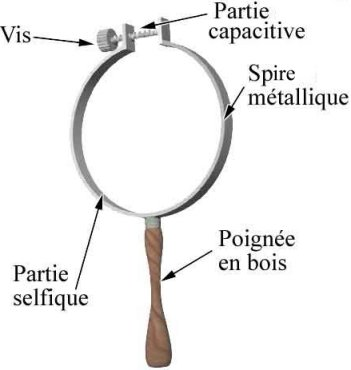
\includegraphics[height=5cm]{hertz1}
		\caption{Récepteur de Hertz}
	\end{minipage}
	\begin{minipage}[]{.5\linewidth}\centering
		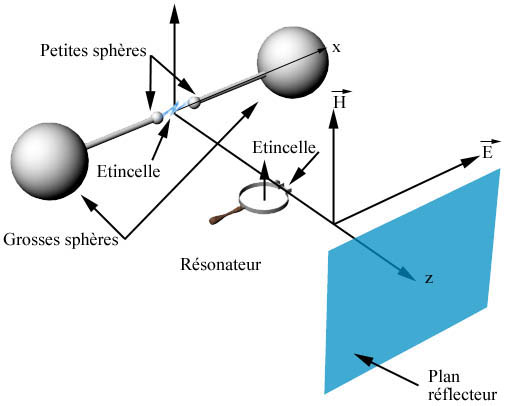
\includegraphics[height=5cm]{hertz2}
		\label{fig:expHertz}
		\caption{Expérience de Hertz} 
	\end{minipage}
\end{figure}

\subsection{Physique du rayonnement}
%Ce paragraphe introductif traite de l'intuition qui se cache derrière les champs rayonnés : il se réfère aux lectures supplémentaires disponibles sur le site du cours. \\ \\
Nous avons vu (en Physique 1 et 2) qu'une charge au repos dans un référentiel galiléen classique crée un champ électrique statique, et qu'une charge en mouvement uniforme (ou un courant continu) génère un champ magnétique statique, on peut montrer qu'une charge accélérée est responsable de l'apparition d'un champ rayonné : une onde électromagnétique. Ce champ rayonné résulte des équations de Maxwell, et intègre donc bien un couplage entre champ magnétique et champ électrique. \\ \\
%Nous nous proposons ici d'expliquer brièvement en quoi, lorsqu'une charge est accélérée, un phénomène de rayonnement apparaît. Il est tout d'abord nécessaire de s'imaginer un champ électrique statique associé à une charge au repos. Admettons que pour une certaine raison, elle soit accélérée uniformément selon la direction $\hat{x}$ du référentiel considéré avec une intensité $a$ pendant un temps $\tau$ à partir de $t = 0$. Après, pour $t>\tau$, l'accélération cesse et la particule continue son bonhomme de chemin à une allure constante $v = a\,\tau$ selon $\hat{x}$. A vitesse constante, la particule développe non seulement un champ magnétique mais également un champ électrique non-plus statique mais en mouvement ; en vulgarisant quelque peu, "\textit{centré et attaché}" à la particule. En considérant les temps $t = 0$ et $t = \tau$, nous observons aisément que le champ électrique associé à la particule chargée n'est pas centré au même endroit : il a non seulement été projeté en avant suite au mouvement de la particule mais ce de manière plus rapide que la vitesse initiale constante de déplacement du champ électrique jusque là (accélération). Le développement suivi ici est donc valable pour toute accélération de la particule chargée : qu'importe sa vitesse initiale. Cependant, et c'est là où réside toute l'essence même du rayonnement, ce changement de \textit{centrage} ne s'opère pas de manière instantanée! La figure \ref{fig:yo} montre bien que "\textit{l'information physique}" se propage à vitesse finie ($c = \frac{1}{\sqrt{\epsilon\,\mu}} < \infty $) vers l'extérieur.
\begin{marginfigure}[1.5cm]
	\centering
	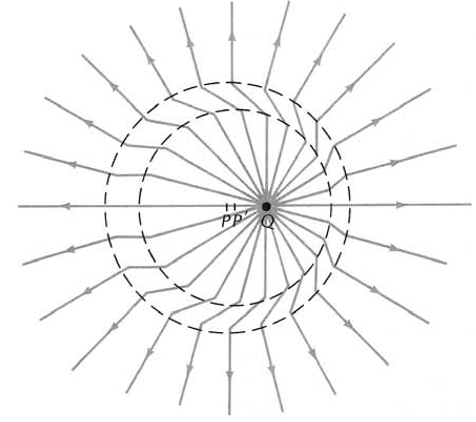
\includegraphics[height=4.3cm]{figure_ray.PNG}
	\caption{Illustration du changement de \textit{centrage} et propagation du signal (tirée des lectures complémentaires). Q est la position actuelle de la charge, P la position initiale. Entre P et P', la charge a subi une accélération, depuis, elle bouge à vitesse constante.}%Pas toute la description, 
	\label{fig:yo2}
\end{marginfigure}


S'il y a propagation d'une onde, le champ rayonné en un point de l'espace $\vec{r}$ dépend bien du champ créé par la charge accélérée au temps $t' = t - \frac{|| \vec{r} - \vec{r}_{p} ||}{c}$. En effet, il faut tenir compte du déphasage temporel $\frac{||\vec{r} - \vec{r}_{p} ||}{c}$ lié au temps mis par le front d'onde pour arriver en $\vec{r}$ depuis $\vec{r}_{p}$ (position de la charge accélérée). \\ \\
Aussi, intuitivement, nous accepterons pour la suite du document que l'amplitude du champ rayonné est directement proportionnelle à l'accélération subie. De plus, il va nous falloir admettre un postulat ; confirmé par la figure \ref{fig:yo} si nous regardons dans la direction de l'accélération. Il s'agit d'observer que seule la composante orthogonale de l'accélération en $t'$ par rapport à la position $\vec{r}$ considérée entraine un rayonnement. Cet effet est illustré à la figure \ref{fig:yo2}. \\ \\
Enfin, puisque la puissance du signal (champ électrique) se propageant doit être conservée et qu'il se propage dans toutes les directions \footnote{Nous verrons qu'il faut être prudent en disant cela : certaines directions se verront doter d'une propagation de champ rayonné d'amplitude nulle. Il est ici juste nécessaire de saisir les idées sous-jacentes.}, il faut savoir que l'intensité ([$W/m^{2}$]) du champ rayonné sera proportionnelle à $\frac{1}{|| \vec{r} - \vec{r_{p}} ||^{2} }$ 
puisque le front d'onde décrit successivement des sphères centrées en $\vec{r}_{p}$ d'enveloppe de surface évoluant avec le carré du rayon. Attendu que, comme nous avons pu le découvrir, l'intensité est directement liée au carré de l'amplitude du champ électrique associé ; cette dernière sera proportionnelle à $\frac{1}{||\vec{r} - \vec{r_{p}}||}$ 

\begin{figure}[h]
	\centering
	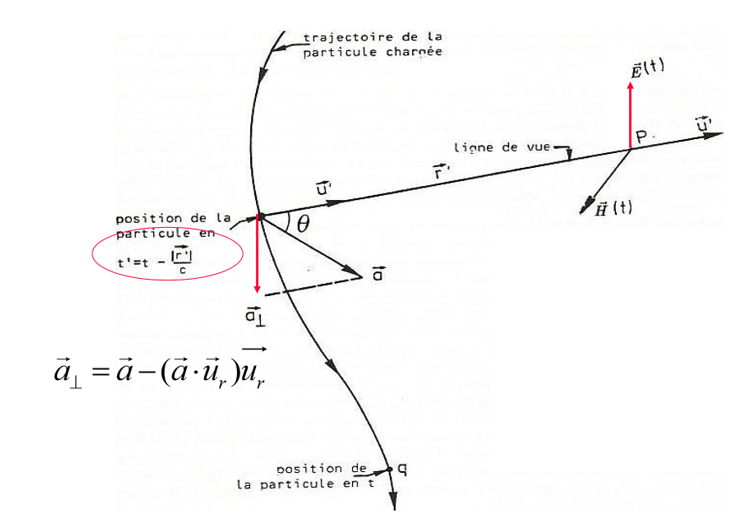
\includegraphics[height=8cm]{lol2.PNG}
	\caption{Illustration du postulat}
	\label{fig:yo2}
\end{figure} 

Au final, en combinant toutes les observations et les hypothèses émises, nous formulons que l'amplitude du champ électrique  rayonné\footnote{Lorsque ce champ électrique rayonné variera dans le temps, là apparaîtra ce fameux couplage à un champ magnétique formant, à deux, une onde E.M. Nous y reviendrons.} suit une proportionnalité du type : 
\[ E_{r}(\vec{r},t) = || \vec{E}_{r}(\vec{r},t) || \propto \frac{q}{r}\,\vec{a}_{\perp}(t' = t - \frac{||\vec{r}-\vec{r}_{p}||}{c})\]

Dans la suite du document, plusieurs abus de notations / simplifications seront utilisés. \\ \\ Premièrement, nous parlerons souvent de champ électrique (sous-entendu : total) à la place de champ électrique rayonné. Cela vient du fait que selon la loi de Coulomb traditionnelle, l'amplitude des champs électriques statiques (ou se déplaçant à vitesse constante) sont, à tout instant, inversement proportionnels au carré de la distance qui sépare un point considéré de l'espace vis-à-vis du centre (la charge). Le champ rayonné quant à lui est "\textit{seulement}" inversement proportionnel à la distance tout court. Autrement dit, lorsque nous sommes relativement éloignés du "\textit{centre}", c'est à dire de la source ponctuelle de champ électrique (particule chargée), l'amplitude du champ électrique de base tend très rapidement vers des quantités tout à fait négligeables devant l'amplitude du champ rayonné ; voilà pourquoi, à distance convenable, nous marquerons souvent : \[\vec{E} \simeq \vec{E}_{r}\] 
Secondement, parfois, certaines formules ne feront pas la distinction entre $t$ et $t'$. \\\\
Enfin, attendu que nous considérerons toujours un dipôle oscillant comme la base de nos champs rayonnés et que les particules chargées dans ce cas là bougent le long d'un axe (antenne) sur de très courtes distances généralement, nous admettrons souvent que $\vec{r}_{p} \simeq \vec{0}$.\sidenote[][-4cm]{Comme annoncé précédemment, une explication plus formelle encore est disponible dans les notes complémentaires du cours. A nouveau, ce n'est pas matière de l'examen. Il est néanmoins intéressant de lire ces documents. Une animation est disponible sur ce site pour mieux visualiser le phénomène de rayonnement : \url{http://www.tapir.caltech.edu/~teviet/Waves/empulse.html}}

\section{Sources de rayonnement élémentaires}
\begin{figure}[h]\centering
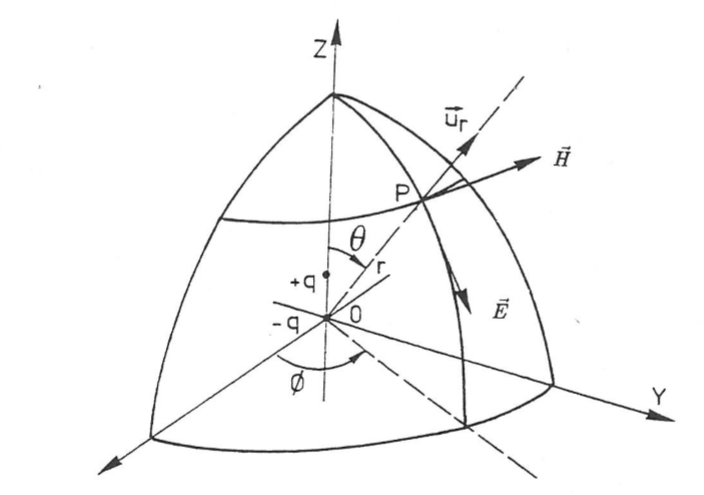
\includegraphics[height=6cm]{radiation.PNG}
%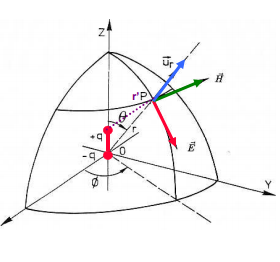
\includegraphics[height=6cm]{dipole} %Celui ci est en couleur
\caption{Représentation de la situation}
\label{fig:dipo}
\end{figure}
Dans le cadre de cette section à propos des sources de rayonnement élémentaires, le modèle simplifié que nous traiterons est le dipôle oscillant formé par une charge négative fixe au centre du repère et une charge positive oscillant selon la trajectoire\sidenote[][-3.5cm]{Il y a une analogie entre cette configuration et le dipôle électrique décrit lors de l'\textit{introduction historique}. Les deux situations suivantes présentent un même moment dipolaire au fil du temps $\Rightarrow$ déplacement combiné d'une charge positive $+\frac{q}{2}$ selon $z_{0}\,\sin (\omega\, t)\hat{z}$ et d'une charge négative $-\frac{q}{2}$ selon $-z_{0}\,\sin (\omega\, t) \hat{z}$ ou charge négative $-q$ fixe en l'origine et déplacement d'une charge positive $+q$ selon $z_{0}\,\sin (\omega\, t)\hat{z}$.} $$ \vec{r}_{p+}(t) = z_{0}\,\sin (\omega\, t) \,\hat{z}$$ 
En plus des simplifications énoncées à la fin de la page précédente, nous émettons certaines hypothèses afin de justifier notre modèle mathématique\sidenote[][-2cm]{Une troisième hypothèse supplémentaire est énoncée dans la lecture suivante \url{http://www.physics.sfsu.edu/~lea/courses/ugrad/460notes5.PDF} où est détaillé, bien davantage qu'ici, un exemple de développement menant à l'expression d'un champ rayonné dans un cas de dipôle oscillant.} :
\begin{enumerate}
\item Le point d'observation est relativement éloigné du dipôle ; \\la distance entre les deux charges puisse être négligée ($r>>z_0$). 
\item L'amplitude d'oscillation est nettement inférieure à la longueur d'onde $\lambda$ de l'onde E.M. émise ($z_0 <<\lambda$). Nous reviendrons sur cette hypothèse.
\end{enumerate}
Ces deux hypothèses impliquent que $r'=r-z\cos(\theta)\simeq r$ et que $\theta'\simeq \theta$.
\subsection{Postulat}
Outre l'intuition sur la relation de proportionnalité suivie par\\ $\vec{E}_{r} \simeq \vec{E}$, nous postulons maintenant\footnote{Forcément, ce n'est pas rigoureusement exact! Nous nous autoriserons cependant à accepter le postulat à suivre muni de son \textit{égalité}. Cette loi se vérifie empiriquement.} que,
$$ \vec{E} = -\frac{1}{4\pi\epsilon_{0}c^2} \,\frac{q}{r'}\,\vec{a}_{\perp}(t')$$

En déduisant, en outre, que $||\vec{r} - \vec{r}_p|| = r' \simeq ||\vec{r}|| = r$. Dans les conditions électromagnétiques physiques du vide, nous réécrivons plus synthétiquement: 

$$ \vec{E} = -\frac{\mu_0}{4\pi} \,\frac{q}{r}\,\vec{a}_{\perp}(t-\frac{r}{c_0})$$
Les formules sont, bien entendu, transposables aux cas d'une transmission hors conditions de vide.

Intéressons nous désormais au champ électrique rayonné en $\vec{r}$ sur base de notre postulat. \\ \\Nous avons choisi un cas particulier pour $\vec{r}_{p+}$ (trajectoire reprenant à chaque instant les endroits où la particule chargée positivement (+) accélère). De manière plus générale, en choisissant $\vec{a}(t) = a(t)\,\hat{z}$, nous réécrivons la relation précédente comme suit : 
$$ \vec{E} = \vec{E}_{\theta} = \frac{\mu_0}{4\pi} \,\frac{q}{r}\,a(t-\frac{r}{c_0}) \, \sin(\theta)\,\hat{e}_{\theta}$$ où le signe $-$ disparaît au profit d'un bon choix de coordonnées sphériques ($\hat{r},\,\hat{e}_{\phi},\,\hat{e}_{\theta}$) (comme spécifié à la figure \ref{fig:dipo}) Le terme $\sin(\theta)$\footnote{Selon nos hypothèses, l'angle $\theta$ est considéré comme constant au cours du temps par rapport au dipôle pour une position $\vec{r}$ donnée.} provient du fait que nous devions nous en tenir à une composante orthogonale au vecteur position $\vec{r}$.\\ \\
Notons avant d'entrer dans des formules \textbf{qu'il ne faut surtout pas} remplacer $t'$ par $t$ car (et c'est le cas de notre exemple) l'accélération est parfois sujette à des changements incessants voire abrupts et il n'est pas envisageable de laisser tomber la précision quant au déphasage de l'onde perçue. \\
Dans ce qui suit, le lecteur peut déduire l'expression du champ magnétique à partir de celle du champ électrique en appliquant $$\vec{H} = \vec{H}_{\phi} = \sqrt{\frac{\epsilon}{\mu}} \, E_{\theta} \, \hat{e}_{\phi}$$
Ici, $a(t) = -z_{0}\,\omega^2\,\sin(\omega\,t)$, d'où \footnote{En étant pointilleux, il faut ajouter que l'expression à venir sera correcte pour les lieux de l'espace pour lesquels le vecteur d'onde $\vec{k}$ est conservé.}  $ a(t-\frac{r'}{c_0}) = -z_0\,\omega^2\,\sin(\omega\,t - k\,r') $
En posant (intensité du moment dipolaire) $p_0 = q\,z_0$, \begin{multline*} \vec{E}_{\theta} = -\frac{\mu_0}{4\,\pi}\,\omega^2\,p_0\,\frac{\sin(\theta)}{r'}\,\sin(\omega\,t - k\,r')\,\hat{e}_{\theta}\simeq \\ \quad -\frac{\mu_0}{4\,\pi}\,\omega^2\,p_0\,\frac{\sin(\theta)}{r}\,\sin(\omega\,t - k\,r)\,\hat{e}_{\theta}\end{multline*}
Cette onde est polarisée \textit{linéairement} selon $\vec{e}_{\theta}$ et, à grande distance du dipôle, nous pourrons considérer que localement nous avons affaire à une onde \textit{plane}.\\
Notons que pour tout point de l'espace, il existera toujours une période transitoire à partir du début de l'oscillation du dipôle pendant laquelle l'équation ci-dessus n'est pas vérifiée (domaine de validité non-encore atteint). La raison du commentaire précédent est laissée aux lecteurs avisés. 

\begin{figure}[h]\centering
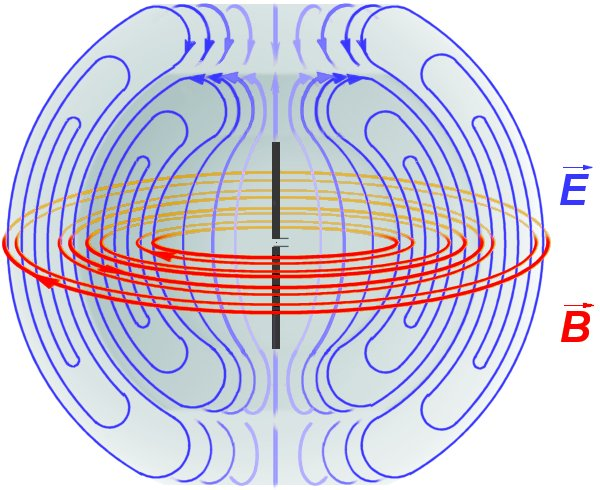
\includegraphics[height=5.8cm]{representation.jpg}
\caption{Champ électromagnétique rayonné par le dipôle}
\label{fig:dipo2}
\end{figure}


\section{Antennes élémentaires}

Désormais, afin de se rapprocher des équations utilisées dans la pratique lorsque nous parlons d'antennes, nous allons construire un parallélisme entre \textit{source de rayonnement élémentaire} et ce que nous dénommerons par \textit{antenne élémentaire}. Dans le cadre des antennes, nous décrirons la source de notre rayonnement par une longueur d'antenne ainsi que l'intensité caractéristique d'un courant la parcourant.
\subsection{Antenne élémentaire de petite taille}
Reprenons l'idée (voire annotation $6$) d'un ensemble de deux charges opposées ($\pm\,q$) décrivant des trajectoires sinusoïdales $\pm\,z_0\,\sin(\omega\,t)$ pour $\vec{r}_{p+}(t)$ et $\vec{r}_{p-}(t)$ respectivement. Par rapport à la situation de la section précédente, il s'agit simplement d'un moment dipolaire $\vec{p}(t)$ double.\footnote{Il y aurait eu équivalence si les charges étaient $\pm\,\frac{q}{2}$.} A partir de ces charges opposées en mouvements sinusoïdaux opposés, nous pouvons esquisser une analogie avec un courant sinusoïdal élémentaire. 

\begin{figure}[h]\centering
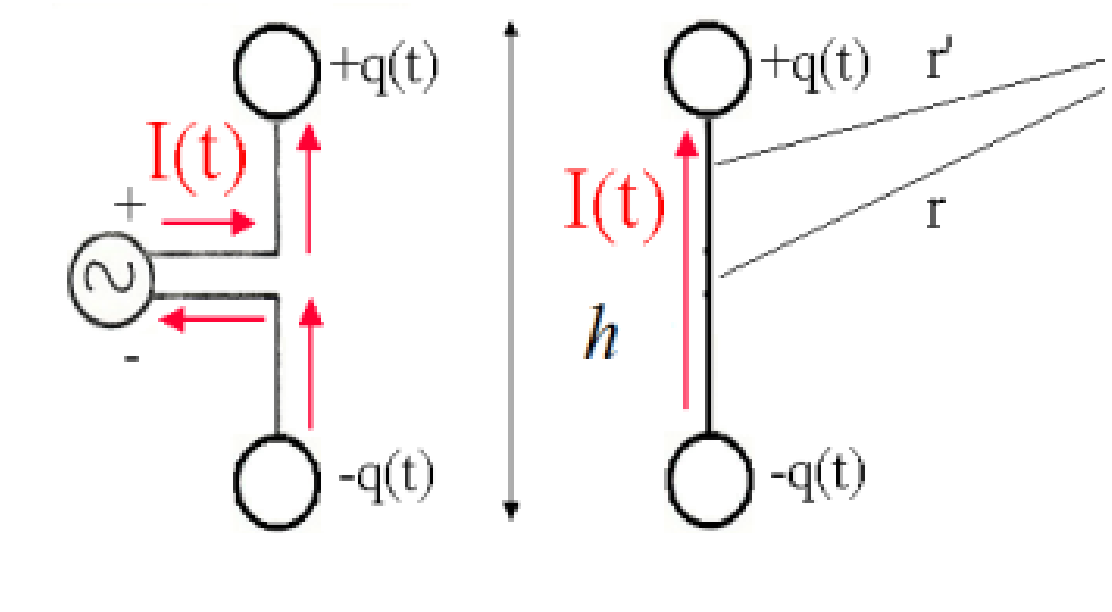
\includegraphics[height=4.2cm]{idea.PNG}
\caption{Illustration tirée des slides montrant l'analogie}
\label{fig:ae}
\end{figure}

Le raisonnement mathématique suivant introduit \textit{grossièrement} \\la transition entre source élémentaire de rayonnement et antenne élémentaire de longueur (petite taille) $ h = \Delta z << \lambda$ : le long de cette antenne élémentaire, les paramètres ($\theta$, $r$ ou $r'$) sont supposés constants et les champs émis en tout point (de $z=-h/2$ jusque $z=h/2$) oscillent en phase.\footnote{La trajectoire prise ici dans les calculs est celle que nous associerons au flot de charges (+) constituant notre \textit{courant}.} \[ I(t) = \frac{\textrm{d}q}{\textrm{d}t} = \frac{\textrm{d}q}{\textrm{d}z}\,\dot\,\frac{\textrm{d}z}{\textrm{d}t}\] Sous hypothèse de courant sinusoïdal avec $\frac{\textrm{d}z}{\textrm{d}t} = \frac{\textrm{d}r_{p+}}{\textrm{d}t}$ :
\[I_{0}\,\cos(\omega\,t) = \frac{\textrm{d}q}{\textrm{d}z}\,\omega\,z_0\,\cos(\omega\,t) \Leftrightarrow I_0\,d\textrm{z} =\omega \, z_0 \textrm{d}q \]
En intégrant donc cette relation tout le long de l'antenne élémentaire (hauteur $h = 2z_0)$, nous obtenons (en faisant l'hypothèse d'un courant constant le long de l'antenne) \[ I_0\,\Delta\,z = I_0 \,h = 2I_0\,z_0 = \omega \,z_0\,\Delta\,q = \omega\, z_0 \, (q-(-q)) = 2\omega\,z_0\,q \Rightarrow I_0\,h = \omega\,p_0\]
Nous pouvons alors écrire pour une antenne élémentaire telle que décrite précédemment : 
\[ E_\theta = -\frac{\mu_0}{4\pi}\omega^2p_0\frac{\sin(\theta)}{r}\sin(\omega t-k\,r)\]
\[ E_\theta = -\frac{\mu_0}{4\pi}\omega I_0h\frac{\sin(\theta)}{r}\sin(\omega t-k\,r) =  -\frac{1}{2}\sqrt{\frac{\mu_0}{\epsilon_0}}I_0 \frac{h}{\lambda}\frac{\sin(\theta)}{r}\sin(\omega t-k\, r)\]



\subsection{Antenne élémentaire de taille quelconque}

Désormais, nous allons tenter de généraliser la formule précédente au cas d'une antenne de taille quelconque : l'hypothèse \\$h<<\lambda$ n'est dès lors plus valide. Il y a dans ce cas une différence de phase non négligeable entre les champs émis en $z=-h/2$ et en $z=h/2$:
$$ r_{h/2}-r_{-h/2}=h\sin(\theta)\Rightarrow \sin(\omega t-kr_{h/2})=\sin\bigg(\omega t-kr_{-h/2}+2\pi\frac{h}{\lambda}\cos(\theta)\bigg)$$
avec $r_{\pm h/2}$ la distance entre l'extrémité de l'antenne ($z=\pm h/2$) et le point $P$. On remarque ainsi que les champs émis aux extrémités de l'antenne seront d'autant plus déphasés que le rapport $h/\lambda$ est élevé. Le déphasage augmente donc progressivement le long de l'antenne.\\
Nous allons procéder à l'intégration de la différentielle suivante selon la coordonnée $z$ : \begin{multline*} \Delta E_{\theta} = -\frac{1}{2}\sqrt{\frac{\mu_0}{\epsilon_0}}I_0 \frac{\Delta z}{\lambda}\frac{\sin(\theta)}{r'}\sin(\omega t-k\, r') \\ \Rightarrow dE_{\theta} = -\frac{1}{2}\sqrt{\frac{\mu_0}{\epsilon_0}}I_0 \frac{\textrm{d}z}{\lambda}\frac{\sin(\theta)}{r'}\sin\Big(\omega t-k\, (r-z\cos(\theta))\Big) \end{multline*}
La longueur $h$ de l'antenne est donc découpée en longueurs infinitésimales $dz$ (voir illustration). Plusieurs simplifications vont désormais être entreprises afin de se donner une formule "\textit{empirique}" approchant bien les résultats en pratique. 

\begin{enumerate}
\item Le point d'observation soit relativement éloigné : par l'approximation de Fraunhofer, nous considérons que $\theta ' \simeq \theta$ même si $h$ est grand.
\item Nous avons $r' = r - z\,\cos(\theta)$ mais le terme $r'$ au dénominateur peut toujours être remplacé par $r$ sans perte de précision exagérée tandis que le terme $k\,r'$ de phase doit être développé en\\ $k\,(r - z\,\cos(\theta))$.
\item Le "\textit{courant caractéristique}" $I_0$ est supposé constant tout le long de l'antenne. 
\end{enumerate}

\begin{figure}[h]\centering
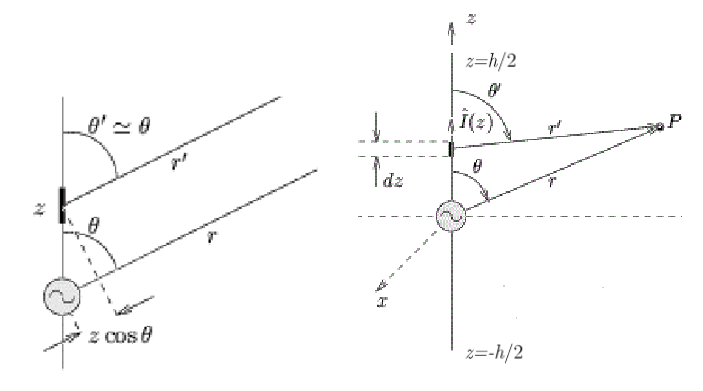
\includegraphics[height=4.5cm]{loll.PNG}
\caption{Illustration tirée des slides décrivant la situation}
\label{fig:ae2}
\end{figure}

Sur base de nos simplifications, nous intégrons légitimement de $z=-\frac{h}{2}$ à $z=\frac{h}{2}$. La manière la plus efficace d'opérer est de passer par les exponentielles complexes $d\bold{E}_{\theta,c}$:
\[ dE_{\theta}=\Re(d\bold{E}_{\theta,c}) =  \Re\bigg(j\,\frac{1}{2}\sqrt{\frac{\mu_0}{\epsilon_0}}I_0 \frac{dz}{\lambda}\frac{\sin(\theta)}{r}e^{j\,(\omega t-k\,(r-z\,\cos(\theta)))}\bigg)\]
en ayant remplacé $r'$ par $r$ au dénominateur.\\ \\
Nous trouvons donc: 

\begin{align*}
\bold{E}_{\theta,c}&=&\int_{-h/2}^{h/2}j\,\frac{1}{2}\sqrt{\frac{\mu_0}{\epsilon_0}}I_0 \frac{\sin(\theta)}{\lambda r}e^{j\,(\omega t-k\,(r-z\,\cos(\theta)))} \mathrm{d}z \\
&=&j\,\frac{1}{2}\sqrt{\frac{\mu_0}{\epsilon_0}}I_0\frac{\sin(\theta)}{\lambda r}e^{j\,(\omega t-kr)} \int_{-h/2}^{h/2}e^{jkz\cos(\theta)} \mathrm{d}z \\
&=&j\,\frac{1}{2}\sqrt{\frac{\mu_0}{\epsilon_0}}I_0\frac{\sin(\theta)}{\lambda r}e^{j\,(\omega t-kr)} \bigg[\frac{e^{jkz\cos(\theta)}}{jk\cos(\theta)}  \bigg]_{-h/2}^{h/2}\\
&=&\frac{1}{2}\sqrt{\frac{\mu_0}{\epsilon_0}}\frac{I_0\sin(\theta)}{k\lambda r\cos(\theta)}e^{j\,(\omega t-kr)} \bigg(e^{jk\frac{h}{2}\cos(\theta)}-e^{-jk\frac{h}{2}\cos(\theta)}\bigg)\\
&=&j\sqrt{\frac{\mu_0}{\epsilon_0}}\frac{I_0}{2\pi r}\tan(\theta)\sin\bigg(\frac{kh}{2}\cos(\theta)\bigg) e^{j\,(\omega t-kr)}\\
&=&\sqrt{\frac{\mu_0}{\epsilon_0}}\frac{I_0}{2\pi r}\tan(\theta)\sin\bigg(\frac{kh}{2}\cos(\theta)\bigg) \Big(j\cos(\omega t-kr)-\sin(\omega t-kr)\Big)
\end{align*}
\[ \Rightarrow E_{\theta} = \Re(\bold{E}_{\theta,c})= -\frac{1}{2\,\pi}\,\sqrt{\frac{\mu_0}{\epsilon_0}}\,\frac{I_0}{r}\,\tan(\theta)\, \sin\bigg(\frac{kh}{2}\,\cos(\theta)\bigg)\,\sin(\omega\,t-k\,r)   \]
En réalité, $I_0$ n'est pas constant le long de notre chemin d'intégration : en première introduction aux télécommunications, nous nous contenterons de cette expression. Notons que la polarisation reste \textit{linéaire}. 



\subsection{Polarisation circulaire}
Comme abordé précédemment dans ce cours, une polarisation \\\textit{circulaire} s'obtiendra facilement à partir d'une combinaison de polarisations \textit{linéaires}. \\ \\Par exemple, en procédant classiquement en développant deux ondes E.M. polarisées linéairement à partir d'antennes places de manière orthogonale (voir illustration) et pour lesquelles les courants sinusoïdaux sont déphasés entre eux de $\frac{\pi}{2}$ en valeur absolue. 

\begin{figure}[h]\centering
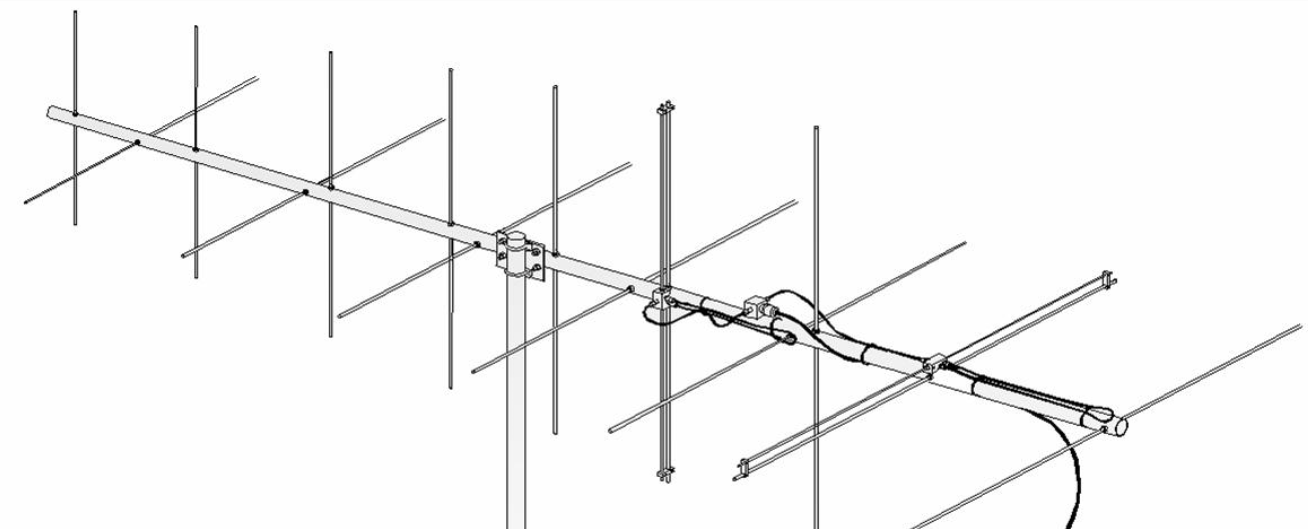
\includegraphics[height=4.5cm]{hehe.PNG}
\caption{Polarisation \textit{circulaire} implémentée par des antennes.}
\label{fig:circ}
\end{figure}

\section{Densité d'énergie rayonnée}

Jusqu'à présent, nous avons observé des schémas classiques de radiation électromagnétique. Attendu que chaque onde électromagnétique soit dotée d'une certaine quantité d'énergie, il est intéressant de développer des schémas de radiation plus complexes afin de diriger les ondes (et donc toute cette énergie, cette information, ... etc) préférentiellement à certains endroits de l'espace.\\ Cette tâche est un exemple concret de problème auquel un ingénieur peut être confronté dans sa vie professionnelle. Nous parlerons dans cette dernière section du concept de densité d'énergie\sidenote{Pour rappel, il s'agit donc du rapport entre énergie transportée par une onde par unité de surface à un endroit donné de l'espace.} véhiculée par une onde.
\begin{marginfigure}
	\centering
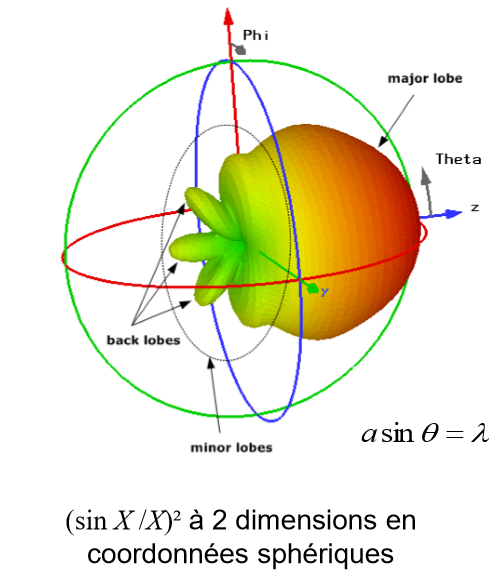
\includegraphics[width=\linewidth]{ex.PNG}
\caption{\textit{Pattern} de radiation électromagnétique plus complexe.}
\label{fig:pattern}
\end{marginfigure}

Nous utiliserons ci-dessous le vecteur de Poynting.\\ Ce vecteur pointe dans la direction de propagation de l'onde électromagnétique et est témoin de l'intensité des champs la formant. 
$$ \vec{S} = \vec{E}\times \vec{H} = \frac{1}{\mu} \vec{E}\times \vec{B} $$
La connaissance de ce dernier en tout point d'une surface permet de calculer un flux d'énergie en sortant, c'est à dire la "\textit{puissance}" sortant de cette surface (appelons la $D$) : 
$$ P = \oiint_{D} \vec{S}\cdot \vec{\textrm{d}s}$$
Si cette surface englobe la source et est fermée, on parle alors de puissance totale émise: 
$$P_{tot}=\oiint_D\vec{S}\cdot \vec{\textrm{d}s}$$
Dans certains cas, il est possible d'obtenir des expressions simplifiés.
Nous définissons dans le cas des ondes planes et dans le cas des ondes sinusoïdaux $I=|\vec{S}|$ la norme du vecteur de Poynting. Ainsi $\vec{S}=I \hat{u}_k$. 
Dans le cas des ondes planes, en utilisant $\vec{H}=\sqrt{\frac{\epsilon_{0}}{\mu_0}}\hat{u}_k \times \vec{E}$, on obtient : 
$$ I=EH=\sqrt{\frac{\epsilon_{0}}{\mu_0}}E^2=\sqrt{\frac{\mu_0}{\epsilon_{0}}}H^2$$
où $E$ et $H$ sont les normes de $\vec{E}$ et $\vec{H}$ respectivement.
Dans le cas des ondes sinusoïdaux, E et H s'expriment de la manière suivante : $E=E_{max}\sin(\omega t-kx)$ et $H=H_{max}\sin(\omega t-kx)=E_{max}^2\sqrt{\frac{\epsilon_0}{\mu_0}}\sin(\omega t-kx)$. Nous définissons en plus l'intensité moyenne:
 
\[\begin{split}
|\vec{S}|_{moy}=I_{moy}&=E_{max}H_{max}\langle \sin^2(\omega t-kx)\rangle \\ &=\frac{E_{max}H_{max}}{2}=\frac{E_{max}^2}{2}\sqrt{\frac{\epsilon_0}{\mu_0}}=\frac{H_{max}^2}{2}\sqrt{\frac{\mu_0}{\epsilon_0}}=\frac{I_{max}}{2}
\end{split}\]
Nous allons maintenant appliquer les éléments ci-dessus à un dipôle, une antenne élémentaire courte et une antenne élémentaire longue pour calculer la puissance moyenne totale pour ces sources. De manière générale, nous devrons calculer 
$$P_{moy}=\oiint \vec{S}_{moy} \cdot \vec{\textrm{d}s} = \oiint I_{moy}\textrm{d}s$$
Les sources élémentaires que nous étudions émettent des ondes sphériques. Nous allons exprimer $I$ en fonction des coordonnées sphériques : 
$$\vec{S}=\vec{E}\times \vec{H}=E_\theta\hat{u_\theta} \times H_\phi\hat{u_\phi}=E_\theta H_\phi\hat{u_r}=\sqrt{\frac{\epsilon_0}{\mu_0}}E_\theta^2\hat{u_r}=\sqrt{\frac{\mu_0}{\epsilon_0}}H_\phi^2\hat{u_r}=I\hat{u_r}$$
\begin{equation}\begin{split}
P_{moy} = \oiint I_{moy}\vec{\textrm{d}s} &= \int_0^{2\pi}\int_0^{\pi} I_{moy}(r\textrm{d}\theta)(r\sin\theta\textrm{d}\phi)\\
&=\int_0^{2\pi}\int_0^{\pi}\sqrt{\frac{\epsilon_{0}}{\mu_0}}\frac{E_{\theta,max}^2}{2}r^2\sin\theta\textrm{d}\theta\textrm{d}\phi
\end{split}\end{equation}
avec le champ électrique
\[E_\theta=\frac{\mu_0}{4\pi}\omega^2p_0\frac{\sin \theta}{r}\sin(\omega t-kr) \hspace{3mm} \Rightarrow \hspace{3mm} E_{\theta,max}=\frac{\mu_0}{4\pi}\omega^2p_0\frac{\sin \theta}{r}.\]
Pour un dipôle, l'intégration donne :
\[\begin{split}
P_{moy}  &= \int_0^{2\pi}\int_0^{\pi} \sqrt{\frac{\epsilon_{0}}{\mu_0}} \frac{\left(\frac{\mu_0}{4\pi}\omega^2p_0\frac{\sin \theta}{r}\right)^2}{2}r^2\sin(\theta) \textrm{d}\theta \textrm{d}\phi \\
&=\left(\frac{\mu_0}{4\pi}\right)^2\sqrt{\frac{\epsilon_{0}}{\mu_0}}\frac{\omega^4p_0^2}{2}\frac{r^2}{r^2}\int_0^{2\pi}\textrm{d}\phi \underbrace{\int_0^{\pi}\sin^3(\theta) \textrm{d}\theta}_{4/3} \\
&=\frac{\mu_0^2}{12\pi}\sqrt{\frac{\epsilon_{0}}{\mu_0}}\omega^4p_0^2\end{split}
\]
Pour une antenne linéaire courte, nous supposons que la longueur de l'antenne est largement inférieure à la longueur d'onde : $h<<\lambda$. Dès lors, nous pouvons utiliser la relation précédente et remplacer $\omega p_0$ par $hI_0$.
\[P_{moy}=\frac{\mu_0^2}{12\pi}\sqrt{\frac{\epsilon_{0}}{\mu_0}}
\omega^2(hI_0)^2=\frac{\pi}{3}\sqrt{\frac{\mu_0}{\epsilon_{0}}}\left(\frac{h}{\lambda}\right)^2I_0^2
\]
Pour une antenne linéaire longue, le champ électrique ne peut pas être assimilé à celui des dipôles. On calcule le champ électrique maximum (sur la variable $t$):
\[E_{\theta,max}=\frac{1}{2\pi}\frac{I_0}{r}\tan \theta\sin\left(\frac{kh}{2}\cos\theta\right).\]
Il faut ensuite résoudre numériquement l'intégrale 
\begin{align*}
P_{moy}&=&\sqrt{\frac{\epsilon_{0}}{\mu_0}}\int_0^{\pi}\int_0^{2\pi}\bigg(\frac{1}{2\pi}\sqrt{\frac{\mu_0}{\epsilon_{0}}}\frac{I_0}{r}\tan \theta\sin\left(\frac{kh}{2}\cos\theta\right)\bigg)^2\frac{r^2}{2}\sin(\theta)\textrm{d}\theta\:\textrm{d}\phi\\
&=&\frac{1}{4\pi} \sqrt{\frac{\mu_0}{\epsilon_{0}}}I_0^2\int_0^{\pi}\frac{\sin^3\theta}{\cos^2\theta}\sin^2\left(\frac{kh}{2}\cos\theta\right)\textrm{d}\theta
\end{align*}
car elle ne possède pas de solution analytique.

\subsection{Champ électrique réfléchi}

\begin{marginfigure}[-2cm]
	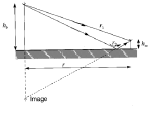
\includegraphics[width=\linewidth]{ant_refl_2}
	\caption{Trajectoire directe $r_1$ et trajectoire comprenant une réflexion $r_2$}
\end{marginfigure}
Nous pouvons aussi calculer la valeur des champs électriques qui ne proviennent pas d'une trajectoire directe. Pour cela, il suffit de calculer le champ électrique avec r qui vaut la distance parcourue par l'onde avant et après la réflexion et multiplier par le coefficient de Fresnel adéquat. Néanmoins, cela nécessite quelques suppositions en plus, l'antenne émettrice doit être linéaire, l'antenne réceptrice doit être isotrope.
\[E_\theta=-\frac{1}{2}\sqrt{\frac{\mu_0}{\epsilon_{0}}}\frac{h}{\lambda}I_0\frac{\sin \theta}{r_{2}}\sin(\omega t-kr_{2})\cdot R_{//}\]
\begin{marginfigure}[-2cm]
	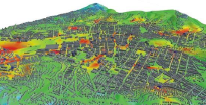
\includegraphics[width=\linewidth]{ant_refl_1}
	\caption{Simulation des intensités des champs électriques du réseau 2G dans la ville de Stuttgart, Allemagne}
\end{marginfigure} 

